% Compact static illustrations of the adjacent worked examples.
\newcommand{\InterpolationFigure}{%
\begin{fig}
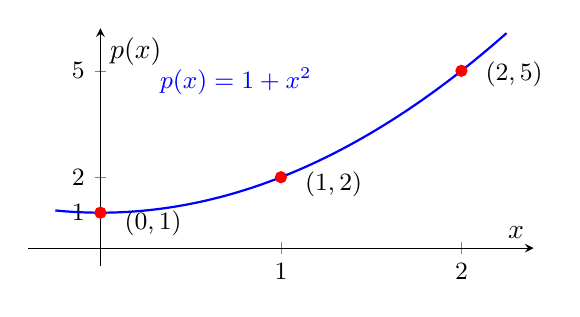
\begin{tikzpicture}
\begin{axis}[width=8cm,height=4.6cm,axis lines=middle,xmin=-.4,xmax=2.4,ymin=-.5,ymax=6.2,xlabel=$x$,ylabel=$p(x)$,xtick={0,1,2},ytick={1,2,5},tick label style={font=\small},clip=false]
\addplot[blue,thick,domain=-.25:2.25,samples=70]{1+x*x};
\addplot[only marks,mark=*,mark size=2pt,red] coordinates{(0,1)(1,2)(2,5)};
\node[anchor=west,font=\small]at(axis cs:.08,.7){$(0,1)$};
\node[anchor=west,font=\small]at(axis cs:1.08,1.8){$(1,2)$};
\node[anchor=west,font=\small]at(axis cs:2.08,4.9){$(2,5)$};
\node[blue,font=\small]at(axis cs:.75,4.7){$p(x)=1+x^2$};
\end{axis}
\end{tikzpicture}
\figcap{Three values at distinct inputs determine one polynomial of degree at most $2$. The computed polynomial passes through all three specified points.}
\end{fig}}
\newcommand{\TransitionFigure}{%
\begin{fig}
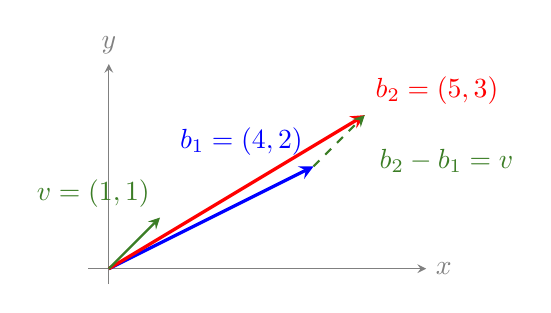
\begin{tikzpicture}[x=.65cm,y=.65cm,>=stealth]
\draw[->,gray](-.4,0)--(6.2,0)node[right]{$x$};
\draw[->,gray](0,-.3)--(0,4)node[above]{$y$};
\draw[->,very thick,blue](0,0)--(4,2)node[above left]{$b_1=(4,2)$};
\draw[->,very thick,red](0,0)--(5,3)node[above right]{$b_2=(5,3)$};
\draw[->,thick,OliveGreen](0,0)--(1,1)node[above left]{$v=(1,1)$};
\draw[->,dashed,OliveGreen,thick](4,2)--(5,3);
\node[OliveGreen,right]at(5.1,2.1){$b_2-b_1=v$};
\end{tikzpicture}
\quad
$\underbrace{\begin{pmatrix}4&5\\2&3\end{pmatrix}}_{Q}
 \underbrace{\binom{-1}{1}}_{[v]_B}
 =\underbrace{\binom{1}{1}}_{[v]_C}$
\figcap{The columns of $Q$ are the $B$-basis vectors written in the standard basis $C$. The same vector $v=b_2-b_1$ has coordinates $(-1,1)$ in $B$ and $(1,1)$ in $C$.}
\end{fig}}
\newcommand{\ProductFigure}{%
\begin{fig}
\[
\begin{aligned}
(1+2x,(3,4))
&=\underbrace{(1,(0,0))+2(x,(0,0))}_{\text{polynomial-coordinate subspace}}\\[-1pt]
&\qquad+\underbrace{3(0,(1,0))+4(0,(0,1))}_{\text{vector-coordinate subspace}}.
\end{aligned}
\]
\figcap{In $\mathcal P_1(\mathbb R)\times\mathbb R^2$, each component contributes its own basis vectors. Reading the two components separately recovers all four coefficients, so the displayed decomposition is unique.}
\end{fig}}
\newcommand{\CosetFigure}{%
\begin{fig}
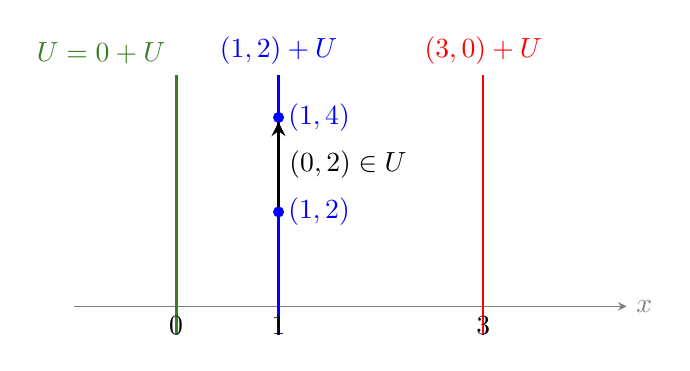
\begin{tikzpicture}[x=1.3cm,y=.6cm,>=stealth]
\draw[->,gray](-1,0)--(4.4,0)node[right]{$x$};
\draw[OliveGreen,very thick](0,-.6)--(0,4.9)node[above left]{$U=0+U$};
\draw[blue,thick](1,-.6)--(1,4.9)node[above]{$(1,2)+U$};
\draw[red,thick](3,-.6)--(3,4.9)node[above]{$(3,0)+U$};
\fill[blue](1,2)circle(2pt)node[right]{$(1,2)$};
\fill[blue](1,4)circle(2pt)node[right]{$(1,4)$};
\draw[->,very thick](1,2.1)--(1,3.9)node[midway,right]{$(0,2)\in U$};
\node[below]at(0,0){$0$};\node[below]at(1,0){$1$};\node[below]at(3,0){$3$};
\end{tikzpicture}
\figcap{For $U=\mathbb R(0,1)$, the two marked representatives give the same blue coset: their difference is in $U$. The red coset is disjoint. The zero vector of the quotient is the entire green line $U$.}
\end{fig}}
